%%NOTES, SCRATCH TEXT
KEEP IN MIND:
-Use Anderson's outside argument for intro.
-Frame this as a question of the trajectory of the prior (not just at end, althought that is potentially most interesting). Here is where can tie into the prior but recent literature on prior changes (from 2014 i think onward).


A complicating issue, one we only raise here for consideration but do not address further, is that In Bayesian decision models, stochasticity can come from different sources  It can come from noise or sampling from the prior, the likelihood, or the decision process itself (the integration of the posterior into the decision process) [REF the magnitude estimation paper for a thorough analysis of these distinctions AND REFRecent work, for example, in a related paradigm (change-point detection) suggests different driving components of human variability,]  We reserve the integration of stochasticity into our rational model for future work, in part because the model doesn't accommodate it.  Instead, our concern is with systematic change that is coupled to external information.

\footnote{For this example, we might assume that the duration of train rides is Poisson distributed (assuming that each ride is an interval and the number of minutes in duration is the number of events). Poisson processes are usually associate with number of events per time interval (e.g., number of failures in 24 hours), but in practice other discrete problems can be modeled as Poisson (e.g., number of trees per acre, number of stock movements per day).  Here we assume events are the number of minutes and the interval is train ride, number of minutes per train ride; for the epidemic case it was the number of days per epidemic wave})


%%FROM OLD DISCUSSION
because The observational context of our data revealed a paradoxical feature of the theoretically driven model of event duration  :  (i) the model generated limiting cases that were both intriguing and not confirmed in prior work; and, (ii) the model did not readily afford the integration of relevant and accessible information.  By transformed the observational data into a form that was amenable to the theoretical model and processing it in a way that revealed the unobservable theoretical components of the model, we provided, in Study 1, a preliminary account of the theoretical model under conditions similar to the limiting cases of interest.  In Study 2, comparing the time-series of the transformed observational data against the epidemiological case count data revealed a strong, sensible relation. 

In totality, the Rational theory and model provided a useful framing of the problem, useful measures and predictive bounds for guiding the interpretation of the results. 

%%%

%%%FROM OLD INTRO
In this work, the experimental manipulation of the prior was based on either verbal scenario manipulation (e.g., describe verbally contextual information related to the prior about the expected duration) or through direct experience in the laboratory. For the latter, participants were provided with direct, controlled experience with relevant materials (see \cite{GriffithsTenenbaum2011} Experiment 4).  In terms of the model, this amounts to manipulation of $P(t_{total})$ through direct experience. 

We can define a Bayesian prediction function (borrowing from \cite{GriffithsTenenbaum2006}) as $t_{predicted}$ over all values of $t_{past}$.  Prior results have shown that, with a Gaussian prior, the Bayesian prediction function is nonlinear: given values of $t_{past}$  $<<$ the mean, the approximate value of $t_{predicted}$ is the mean; however, as $t_{past}$ approaches the mean value of the prior, the value of $t_{predicted}$ increases to values larger than the mean value of the prior.  Once $t_{past}$ is past the mean it converges to $t_{predicted}$ slowly (see Figure 1 of \cite{GriffithsTenenbaum2006}).  

This prediction function accords with human predictions under experimental conditions \citep{GriffithsTenenbaum2006} in which human predictions are provided in reference to a single event (e.g., ask participants to judge how long a train ride will last if a person has been sitting on a train for 20 minutes).





%%%OLD FIGURES ETC.
%Figure \ref{fig:TheoryHeatMap}   
%\begin{figure}
%    \centering
%    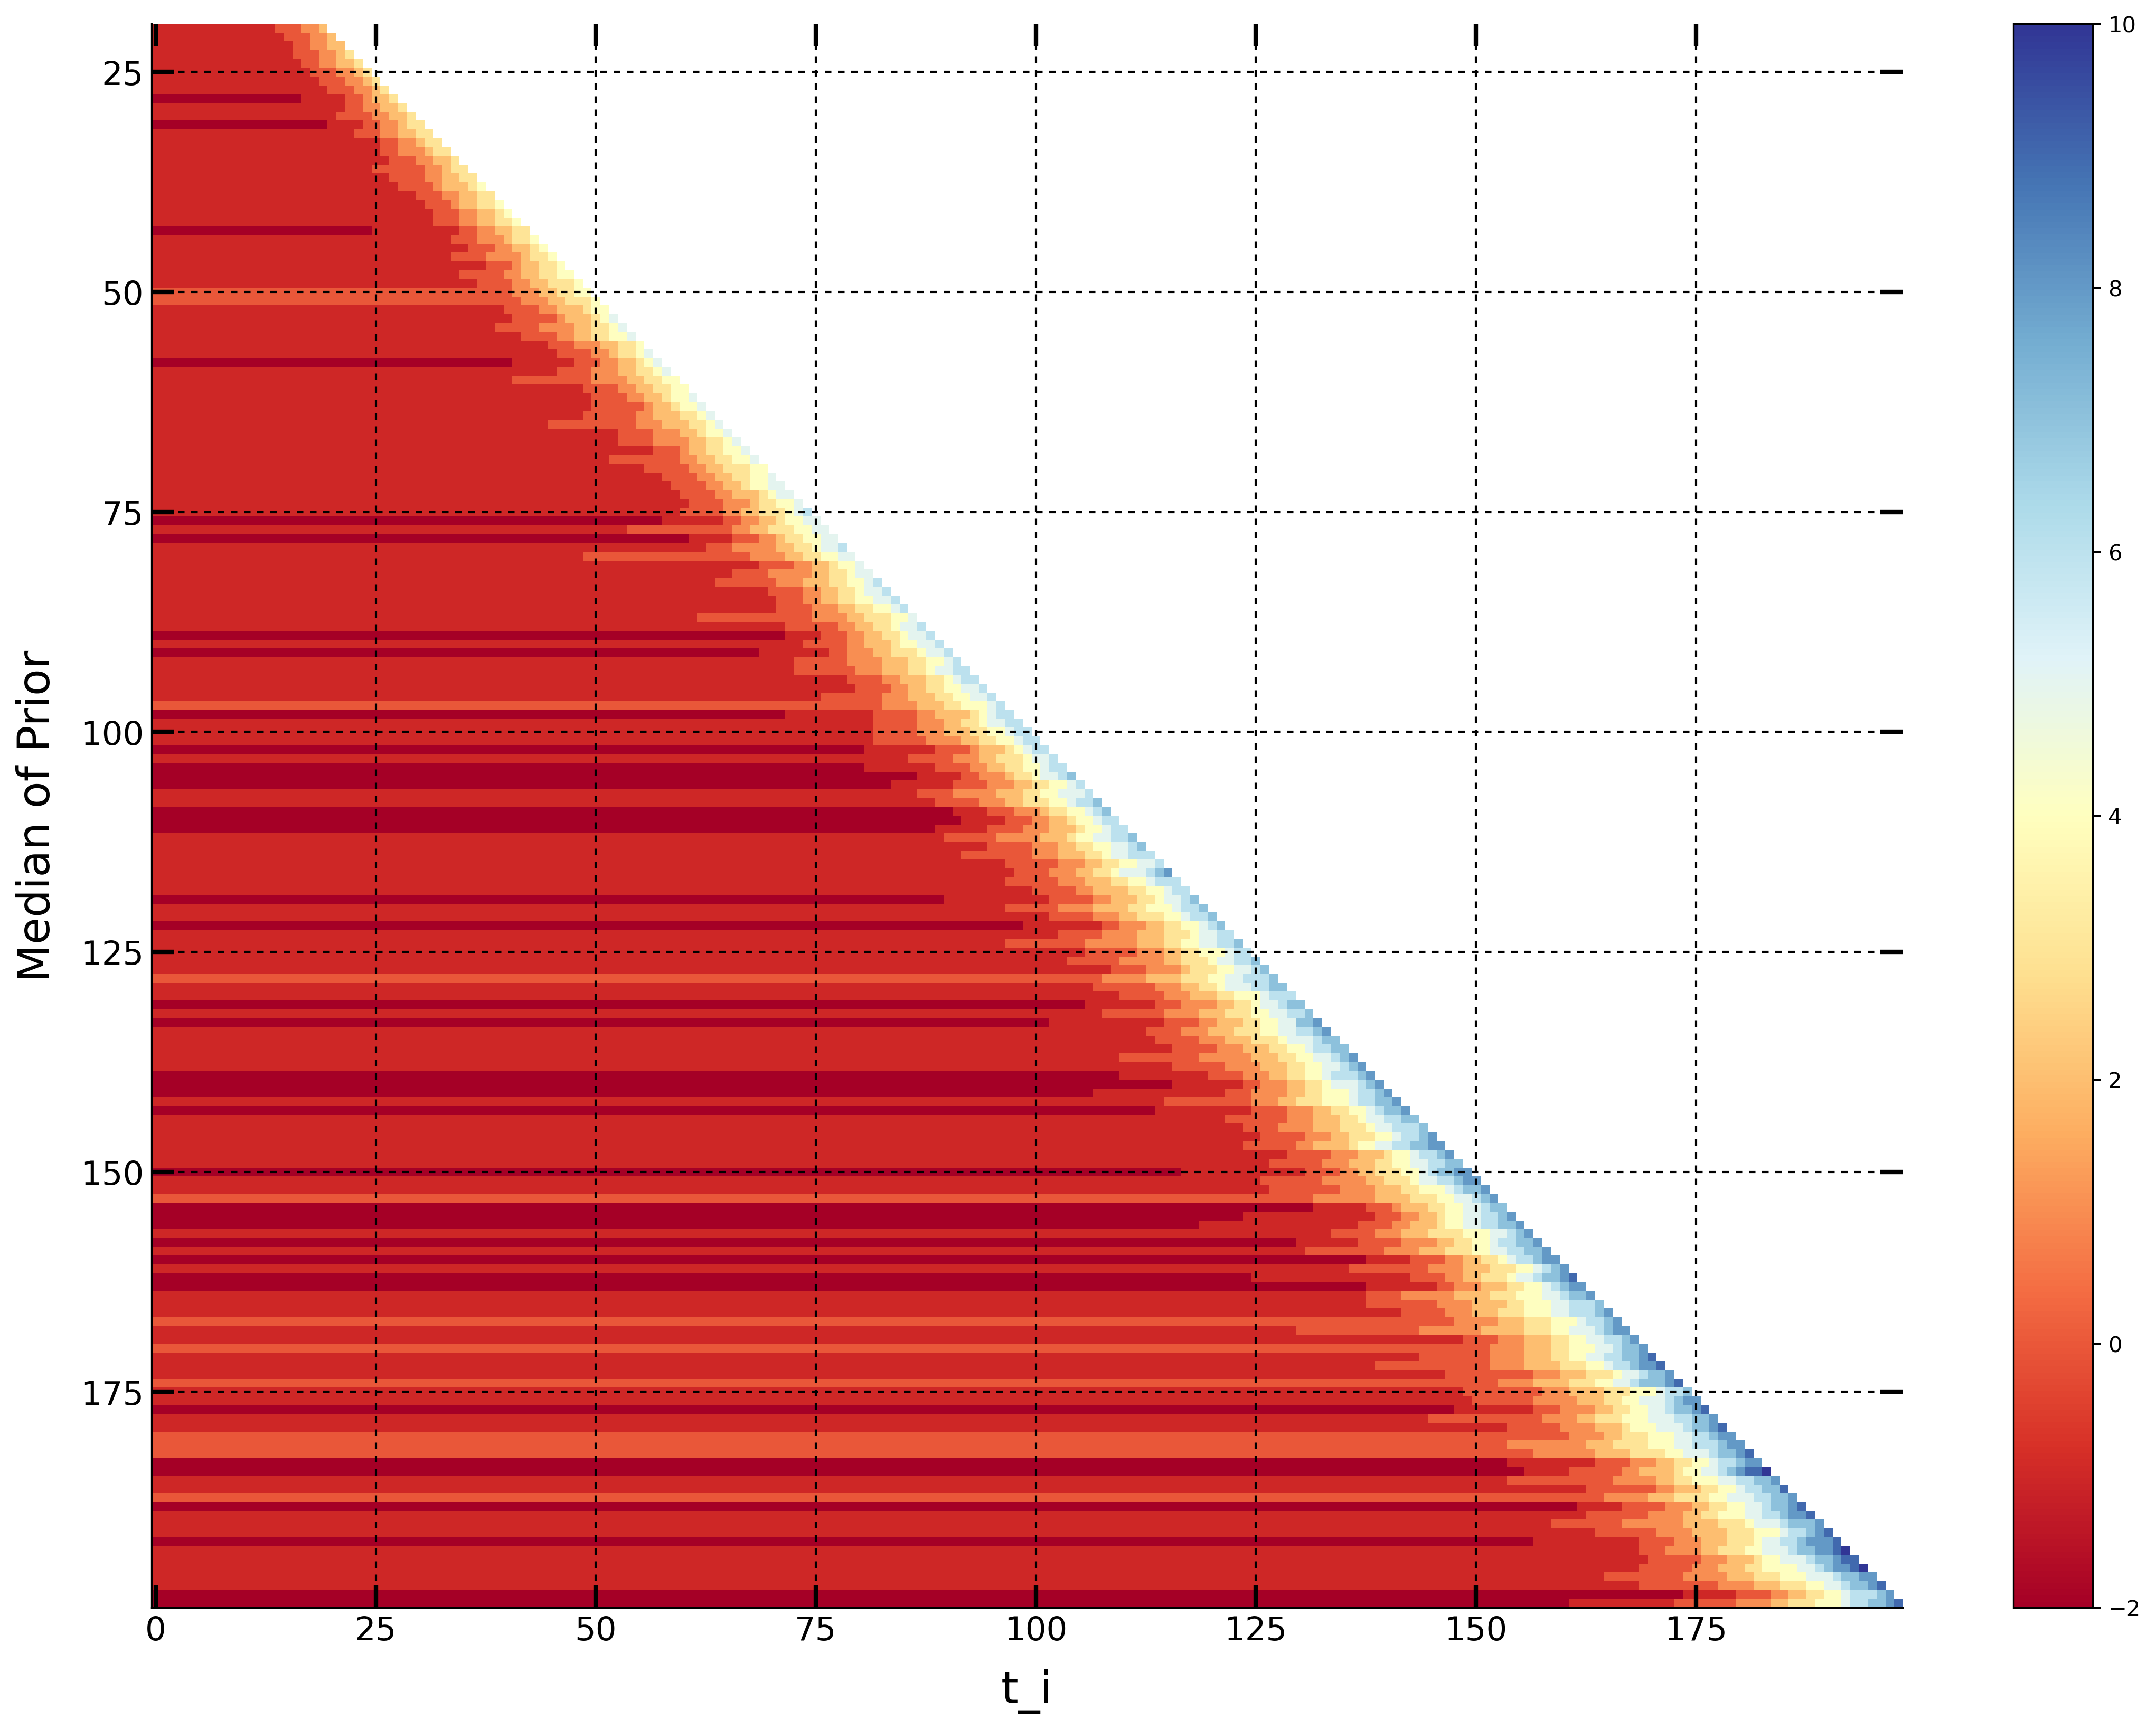
\includegraphics[width=\linewidth]{Figures/TheoryHeatMap_1.png}
%    \caption{The x-axis shows $t_i$; the y-axis shows the median of the prior used in a decision (is the same as $t_{total}$).  The heatmap values were computed as the median of the posterior given a prior distribution and $t_i$ minus the median of the prior.  The key point of this graphic is depicted by the yellow and blue bands:  this shows that as $t_i$ approaches the median of the prior, the estimate of $t_{total}$ increases. To read this graphic, pick a value for median of prior (on the y-axis) and follow it from left-to-right (to simulate increasing $t_i$). 
%    }
%    \label{fig:TheoryHeatMap}
%\end{figure}

%%%REPLY TO CHRIS AND MADHAV

 


I was also thinking along these lines, as it is the natural thing to do.  However, the tack I took with the paper in its current form was to to precisely NOT do this; maybe its more accurate to say completely AVOID doing this.  

This paper was targeted at a journal that takes short articles that have interesting things to say about psychological models or theory.  The interest in this paper comes from the application of the theoretical model to real-world observations in a context that is important to society (COVID).  Its a case study of sorts.  WHat can you learn from applying a mathematical model to observational data?  Does it seem to have enough meat on it for other psychologists to use a similar approach? Not in the narrow scope of our model or the observational domain or of the so-called event duration estimates, but in the general sense.   Maybe what is not clear here is that the field of psychology that deals with mathematical or computational models of cognition is largely not in the practice of putting theory/models into the real-world.  This article offers an example of it that was useful in scientific practice.  

I can't stress this enough, this is the objective for this journal.  Your suggestion here, as I said, is the obvious clear next step.  But that is for another article.  

An alternative, of course, is that we could target another more specialized journal, one that allows for and expects more development in the modeling.  I have no objection to doing this, but I thought we were in a hurry so I put this together in its current form for a top-visibility journal that might go for just the observational part as explained above.  

If we want to pursue a more specialized journal (e.g., Cognitive Science, Cognition) then we could leverage the result from Study 2 (the relation between human predictions and the case counts) as a potential input to the decision model in real-time. 

But, let me push one more time to not do this.  I think the merits of the appraoch, as I state above, will win the day.  There are caveats, see below for two core examples, but these could be preempted in the methods and results sections.


In terms of getting hammered in review, I think these are the core issues:
1. The methodology of recovering the prior from the person's prediction is defensible with one clear weak point:  we assert the beginning of the time horizon as the beginning of the epidemic, call it t_0, with little reasoning except to say that it looks reasonable.  However, notice that we can defend this assertion because error in t_0 is not very consequential for the objective and results.  Study 1 results would be similar even if we were off by so many days, plus or minus.

2. Fixing t_0 and solving for the prior is our approach.  Why not fix the prior and solve for t_0?   Wouldn't it make more sense for folks to think their estimate of t_0 was wrong as in:  "hey, i thought this epidemic wave started 20 days ago, but i guess I was wrong.  It must have started earlier".   I did some development work on this thread, but found it, well, icky.  

Some minor issues in review will be as you stated.

We could figure out how to address these pre-emptively in the methods and results sections (as these do not have limits on length).



TO DO:
Send paper to Austerweil and Goldstone or meet with them.